\documentclass{tufte-handout} % A4 paper and 11pt font size
\usepackage[activate={true,nocompatibility},final,tracking=true,kerning=true,spacing=true,factor=1100,stretch=10,shrink=10]{microtype}
\usepackage[T1]{fontenc} % Use 8-bit encoding that has 256 glyphs
%\usepackage{mathpazo} % Use the Adobe Utopia font for the document - comment this line to return to the LaTeX default
\usepackage[english, serbianc]{babel} % English language/hyphenation


\usepackage{amsmath,amsfonts,amsthm, amssymb} % Math packages
\usepackage{pgf,tikz}
\usetikzlibrary{positioning,matrix,arrows}
\usepackage{float}
\usepackage{tikz-cd}
\usepackage{caption}
\usepackage{stmaryrd}
\usepackage{multicol}
\usepackage{booktabs}
\usepackage{verbatim}
\usepackage{lipsum} % Used for inserting dummy 'Lorem ipsum' text into the template
\usepackage{sectsty} % Allows customizing section commands
\usepackage{titlesec}
\usepackage{empheq}
\usepackage[most]{tcolorbox}
\usepackage{hyperref}
\hypersetup{
	colorlinks = true,
}

\usepackage{mdframed}
\usepackage{tikzsymbols}
\usepackage[makeroom]{cancel}
\usepackage{lmodern}
%Boxed eqns
\newcommand{\boxedeq}[1]{\begin{empheq}[box={\fboxsep=6pt\fbox}]{align} #1\end{empheq}}
\newtcbox{\boxzadatak}[1][]{%
	nobeforeafter, math upper, tcbox raise base,
	enhanced, colframe=blue!30!black,
	colback=blue!30, boxrule=1pt,
	#1}

\tcbuselibrary{theorems}
\newtcbtheorem[number within=section]{zadatak}{Zadatak}%
{colframe=blue!50!black,colback=blue!5,
	colbacktitle=blue!50,colupper=red!35!black,fonttitle=\bfseries}{zz}
\allsectionsfont{\normalfont \bfseries} % Make all sections centered, the default font and small caps
\usepackage{enumerate}
\usepackage{pythonhighlight}
\usepackage{fancyhdr} % Custom headers and footers
\pagestyle{fancyplain} % Makes all pages in the document conform to the custom headers and footers
\fancyhead{} % No page header - if you want one, create it in the same way as the footers below
\fancyfoot[L]{} % Empty left footer
\fancyfoot[C]{} % Empty center footer
\fancyfoot[R]{\thepage} % Page numbering for right footer
\renewcommand{\headrulewidth}{0pt} % Remove header underlines
\renewcommand{\footrulewidth}{0pt} % Remove footer underlines
\setlength{\headheight}{13.6pt} % Customize the height of the header
\allowdisplaybreaks

\usepackage{wrapfig}
\graphicspath{ {./slike/} }

%Sections

%--------Theorem Environments--------
%theoremstyle{plain} --- default
\newtheorem{thm}{Theorem}
\newtheorem{cor}[thm]{Corollary}
\newtheorem{prop}[thm]{Proposition}
\newtheorem{facts}[thm]{Facts}
\newtheorem{fact}[thm]{Fact}
\newtheorem{clm}[thm]{Claim}
\newtheorem{lem}[thm]{Lemma}
\newtheorem{conj}[thm]{Conjecture}
\newtheorem{quest}[thm]{Question}


\theoremstyle{definition}
\newtheorem{defn}[thm]{Definition}
\newtheorem{defns}[thm]{Definitions}
\newtheorem{con}[thm]{Construction}
\newtheorem{exmp}[thm]{Example}
\newtheorem{exmps}[thm]{Examples}
\newtheorem{notn}[thm]{Notation}
\newtheorem{notns}[thm]{Notations}
\newtheorem{addm}[thm]{Addendum}
\newtheorem{zad}[thm]{Zadatak}


\theoremstyle{remark}
\newtheorem{rem}[thm]{Remark}
\newtheorem{rems}[thm]{Remarks}
\newtheorem{warn}[thm]{Warning}
\newtheorem{sch}[thm]{Scholium}


\newcommand{\bra}[1]{\left(#1\right)}
\newcommand{\sbra}[1]{\left[#1\right]}
\newcommand{\Mod}[1]{\ (\text{mod}\ #1)}
\newcommand{\op}[1]{#1^{\text{op}}}
\newcommand{\R}{\mathbb{R}}
\newcommand{\N}{\mathbb{N}}
\newcommand{\Z}{\mathbb{Z}}
%\newcommand{\mZ}{\mathcal{Z}}
\renewcommand{\C}{\mathbb{C}}
\newcommand{\Q}{\mathbb{Q}}
%\newcommand{\F}{\mathbb{F}}
%\newcommand{\bA}{\mathbb{A}}
%\newcommand{\bH}{\mathbb{H}}
\newcommand{\one}{\mathbb{1}}
%\newcommand{\mC}{\mathcal{C}}
%\newcommand{\mO}{\mathcal{O}}
%\newcommand{\mR}{\mathcal{R}}
%\newcommand{\mS}{\mathcal{S}}
%\newcommand{\lp}{{\mathfrak{p}}}
%\renewcommand{\P}{\mathbb{P}}
%\newcommand{\E}{\mathbb{E}}
%\DeclareMathOperator{\dist}{dist}
%\DeclareMathOperator{\aut}{Aut}
%\DeclareMathOperator{\gal}{Gal}
%\DeclareMathOperator{\var}{\textbf{var}}
%\DeclareMathOperator{\orb}{Orb}
%\DeclareMathOperator{\ff}{Frac}
%\DeclareMathOperator{\stab}{Stab}
%\DeclareMathOperator{\inn}{Inn}
%\DeclareMathOperator{\Ind}{Ind}
%\DeclareMathOperator{\Res}{Res}
%\DeclareMathOperator{\spn}{Span}
%\DeclareMathOperator{\out}{Out}
\DeclareMathOperator{\im}{Im}
%\DeclareMathOperator{\rk}{rk}
%\DeclareMathOperator{\disc}{disc}
%\DeclareMathOperator{\tors}{Tors}
%\DeclareMathOperator{\Mor}{Mor}
%\DeclareMathOperator{\End}{End}
%\DeclareMathOperator{\Hom}{Hom}
%\DeclareMathOperator{\Nat}{Nat}
%\DeclareMathOperator{\spec}{Spec}
%\DeclareMathOperator{\ann}{Ann}
%\DeclareMathOperator{\ord}{ord}
%\DeclareMathOperator{\conjc}{Conj}
%\DeclareMathOperator{\Br}{Br}
%\DeclareMathOperator{\Tr}{Tr}
%\DeclareMathOperator{\Nm}{Nm}
%\DeclareMathOperator{\Char}{char}
\newcommand{\norm}[1]{\left\lVert #1 \right\rVert}
\newcommand{\inp}[2]{\left\langle #1, #2 \right\rangle}
\newcommand{\shreq}[2]{-\frac{\hb^2}{2m}\frac{\partial^2 #1}{\partial #2^2} + U(#2) #1 =E #1}
\newcommand{\tshreq}[2]{i\hb\frac{\partial #1}{\partial t^2} = -\frac{\hb^2}{2m}\frac{\partial^2 #1}{\partial #2^2} + U(#2) #1}
\newcommand{\kpsi}{\psi^{''}+k\psi=0}
\def \v {\vspace{0.2cm}}
\newcommand{\hb}{\hslash}
\geometry{
	left=13mm, % left margin
	textwidth=130mm, % main text block
	marginparsep=8mm, % gutter between main text block and margin notes
	marginparwidth=55mm % width of margin notes
}
\fontsize{10}{20}\selectfont
%----------------------------------------------------------------------------------------
%	TITLE SECTION
%----------------------------------------------------------------------------------------

\title{	
	\normalfont\normalsize 
	{Електротехнички факултет, Универзитет у Београду - Летњи семестар 2023.} \\ [0pt] % Your university, school and/or department name(s)
	\huge Белешке - Квантна Механика% The assignment title
}\author{Михаило Стојковић} % Your name
\date{\vspace{-5pt}\normalsize\today} % Today's date or a custom date


\titleformat{\section}
	{}{\noindent\rule{\textwidth}{0.5pt}\\thesection\\\noindent\rule{\textwidth}{0.5pt} }{1em}{}[{\titlerule[0.8pt]}]


\begin{document}
\justifying 
\maketitle

\tableofcontents
\newpage
\vspace{1em}
\hrule
\section{Предавање - 8.3.2023.}
\hrule
\vspace{1em}
Само предавање креће са тим да посматрамо стационарну Шредингерову једначину:
	\boxedeq{\shreq{\psi}{x}}
али у случају када је $U(x)=0$. Заменом $k^2\equiv\frac{2mE}{\hslash^2}$ у претходну једначину\footnote{Оваква смена се често појављује у курсу тако да после неког времена постане стандардно да када год се појави неко $k$ сматрамо да је једнако наведеном изразу} добијамо диференцијалну једначину:
	\boxedeq{\label{eqn:sred_k}\kpsi}
Решење ове диференцијалне једначине можемо изразити у два облика:
\begin{enumerate}
	\item Као збир експоненцијала\footnote{Овај облик решења је јако користан у ситуацијама где нам се Шредингерова једначина сведе на облик сличан једначини (\ref{eqn:sred_k}), где ако је испред коефицијента уз $\psi$ знак минус, функција ће бити чисто реална. Решења у овом облику се често узимају у ситуацијама где разматрамо константну потенцијалну енергију или честицу која се налази у коначној баријери}: $\psi(x)=Ae^{ikx} + Be^{-ikx}$
	\item Као збир синуса и косинуса\footnote{Овај облик решења је јако користан ако на интервалу решавања имамо неку бесконачну баријеру}: $\psi(x)=C\sin(kx)+D\cos(kx)$
\end{enumerate}
Оба облика су решење дате диференцијалне једначине и може се лако показати како једно можемо представити преко другог.\par
Посматрамо решење у експоненцијалном облику. Због хомогености диференцијалне једначине, негативно и позитивно решење можемо посматрати као два засебна решења са додатом функцијом времена.
\begin{align}
	\label{eqn:talas_u_desno}\psi_1(x,t)&=A_1e^{i(kx-\omega t)}\\
	\label{eqn:talas_u_levo}\psi_2(x,t)&=B_1e^{-i(kx-\omega t)} 
\end{align}
и заправо, једначина (\ref{eqn:talas_u_desno}) представља талас који се креће на десно, а једначина (\ref{eqn:talas_u_levo}) представља талас који се креће на лево\footnote{Смер кретања таласа можемо одредити преко \hyperref[]{струје вероватноће}}.

\begin{wrapfigure}{L}{0.5\textwidth}
	\centering
	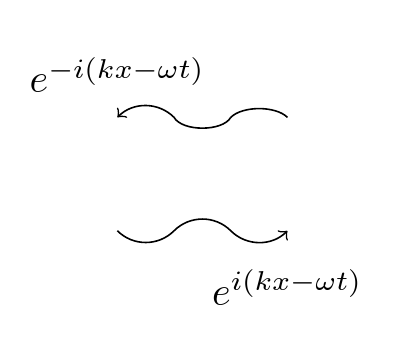
\includegraphics[width=0.5\textwidth]{kretanje_talasa.png}
	\caption{Кретање таласа}
\end{wrapfigure}
Питање које се увек поставља при добитку неког решења једначине: "Да ли ово може представљати таласну једначину". Услови који морају бити испуњени за таласну функцију на неком интервалу су следећи:
\begin{enumerate}
	\item Таласна функција мора бити нормирана\footnote{Погледати (\hyperref[sec:uslov_normiranosti]{Услов нормираности})}
	\item Таласна функција мора бити непрекидна
	\item Први извод таласна функције мора бити непрекидан
\end{enumerate}
При почетку решавања проблема нисмо експлицитно специфицирали интервал решавања, тако да сматрамо да је интервал цело поље $\R$. Овде настаје сада проблем јер решење које смо добили не може да се нормира.
\begin{align}
	\int_{-\infty}^{+\infty}\psi_1^{\ast}\psi_1 dx = |A_1|^2\int_{-\infty}^{+\infty}dx\nless \infty\\ 
	\int_{-\infty}^{+\infty}\psi_2^{\ast}\psi_2 dx = |B_1|^2\int_{-\infty}^{+\infty}dx\nless \infty
\end{align}

Начин на који ово решавамо је мало шкакљив. Претпоставимо да потенцијална енергија није свуда нула, већ само на интервалу $(-\frac{L}{2},\frac{L}{2})$. Ван тог интервала сматрамо да је потенцијална енергија бесконачна, то јест, да честица сигурно мора да се налази на овом интервалу. Ван овог интервала $\psi(x,t)=0$. Бирамо сада функцију (\ref{eqn:talas_u_desno}), без додате функције времена и проверавамо да ли сада можемо да је нормирамо.

\begin{align*}
	&\displaystyle\int_{-\infty}^{+\infty}\norm{\psi_1}^2dx =1\\
	&\displaystyle|A_1|^2\int_{-\frac{L}{2}}^{\frac{L}{2}}|e^{ikx}|^2dx= 1\\
	&|A_1|^2 \cdot L = 1 \implies A_1 = \frac{1}{\sqrt{L}}
\end{align*}
\begin{wrapfigure}{l}{0.5\textwidth}
	\centering
	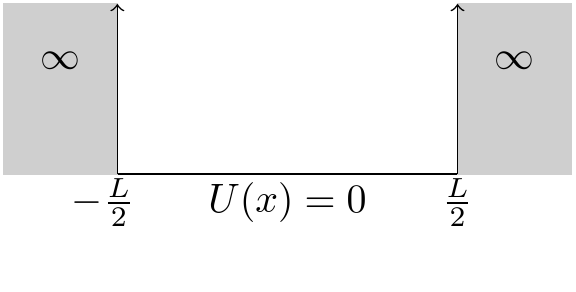
\includegraphics[width=0.5\textwidth]{beskonacne_barijere.png}
	\caption{График потенцијалних баријера. У интервалу $\left(-\frac{L}{2}, \frac{L}{2}\right)$ потенцијална енергија је једнака 0. Ван тог интервала потенцијална енергија је једнака $\infty$}
\end{wrapfigure}
Овим смо добили константу нормирања. Истим поступком можемо добити $B_1$ за једначину (\ref{eqn:talas_u_levo}) и испоставиће се да је једнака $A_1$. Тако да сада имамо решења функција у облику:
\begin{align}
		\psi_1(x)&=\frac{1}{\sqrt{L}}e^{ikx}\\
		\psi_2(x)&=\frac{1}{\sqrt{L}}e^{-ikx} 
\end{align}
Наравно, како би повратили наш првобитни случај, захтевамо да $L\rightarrow\infty$. 

Како би проблем у потпуности решили, морамо да сазнамо какав је спектар енергија. Услов који постављамо за проблеме овог типа(проблеми где уводимо фиктивне границе које теже бесконачности) је да сама функција има исте вредности на оба краја граница.
\begin{align*}
	&\psi_1\left(\frac{L}{2}\right)=\psi_1\left(-\frac{L}{2}\right)\\
	&e^{ik\frac{L}{2}}=e^{-ik\frac{L}{2}}\\
	&e^{ikL}=1
\end{align*}
\begin{figure}[h!]
	\centering
	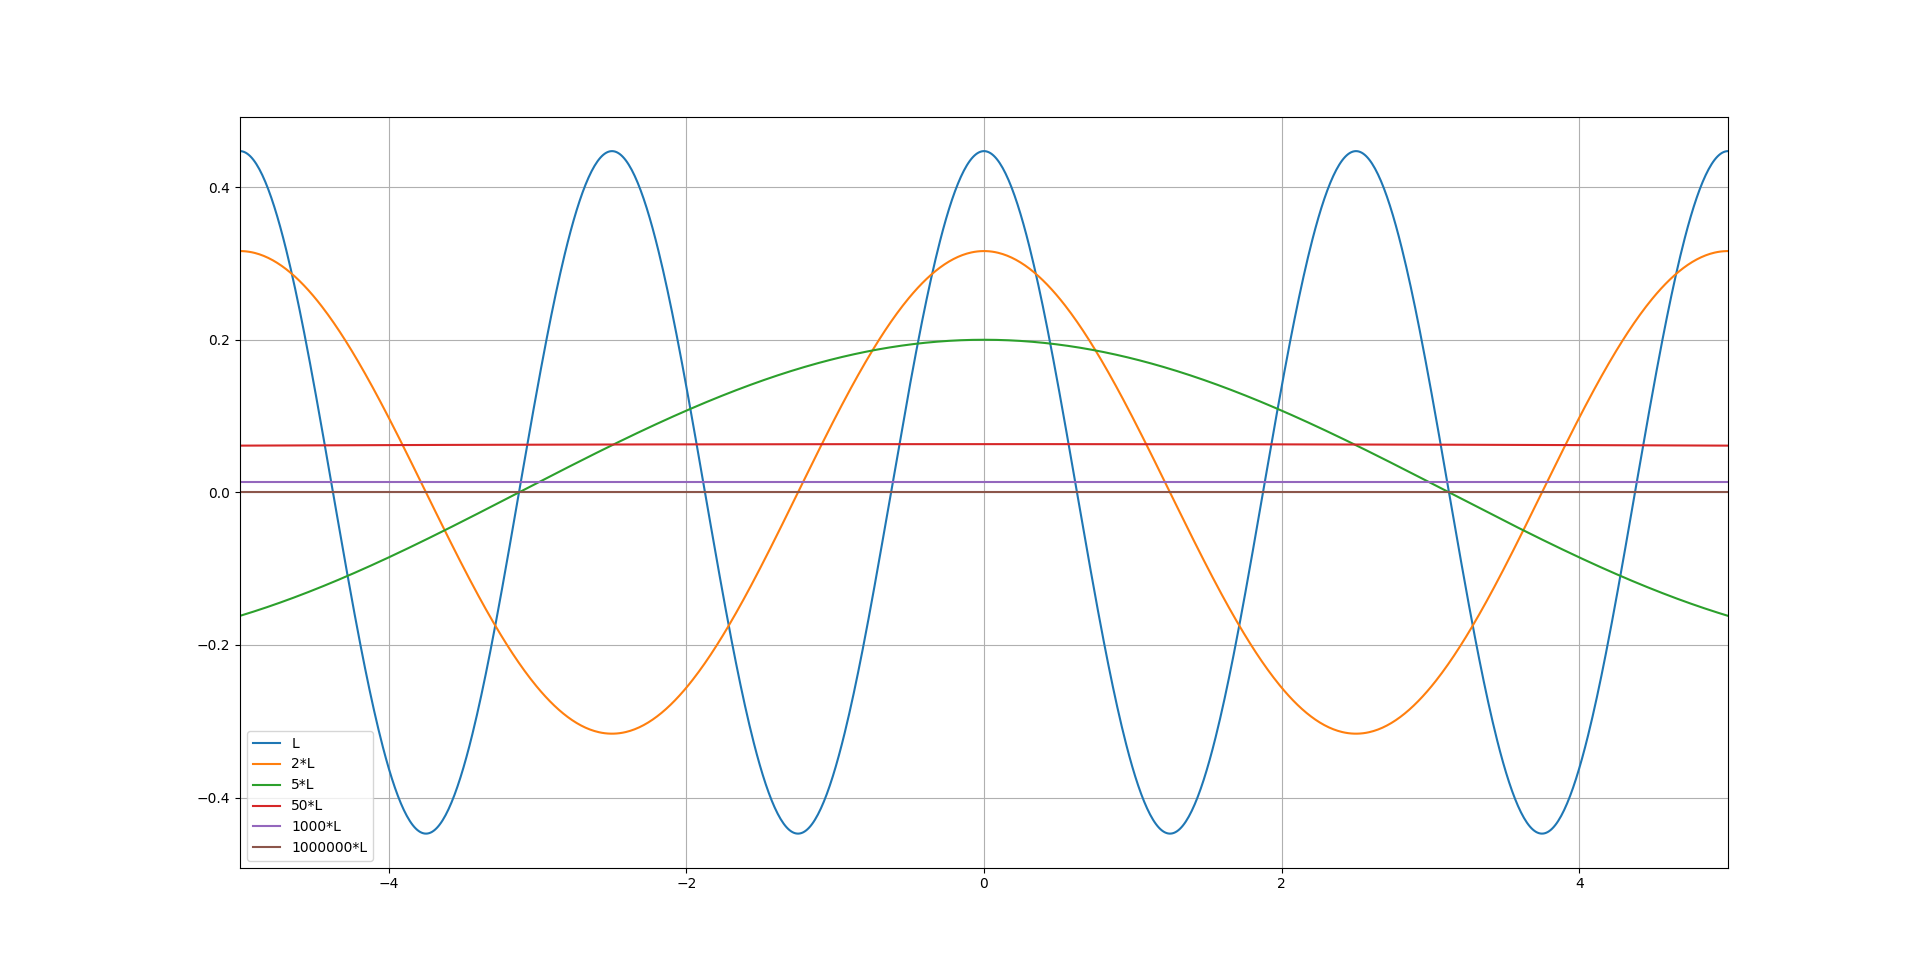
\includegraphics[width=1\textwidth]{grafik_kosinus.png}
	\caption{Графички приказ реалног дела таласне функције $\psi(x)=\frac{1}{\sqrt{L}}e^{ikx}$ са повећањем границе $L$}
\end{figure}
Из последње релације можемо да одредимо вредност $k$ и самим тим и вредност $E$. Овде је битно назначити главни детаљ код оваквих проблема: Увођењем граница довели смо до тога да је спектар дискретан. Једино у граничном случају када баријере теже бесконачности ће се спектар "претворити" у континуалан. Из овога такође закључујемо да проблеми овог типа (без граница) поседују континуални спектар.\par
Додатан детаљ: Ако покушамо да наћемо исти услов за талас који се креће у лево, добићемо идентичну релацију. Одатле закључујемо да у оваквом континуалном спектру постоје две таласне функције које одговарају истој енергији. Број таласних функција у континуалном домену спектра које одговарају истој вредности енергије се назива дегенерација спектра\footnote{У случају који смо разматрали, имамо двоструко дегенерисани континуални спектар}.
\vspace{3em}
\hrule
\subsection*{Слободна честица на полубесконачном домену}
\hrule
\vspace{1em}
Није нигде експлицитно поменуто у претходном делу, али у квантној сматрамо да најмања могућа енергија која честица може да поседује је једнака минималној потенцијалној енергији. С обзиром да потенцијална енергија може да се постави увек тако да јој минимална енергија буде 0, сматрамо да је $E>0$.\par

Посматрамо сада потенцијалну енергију као на слици (\ref{fig:bolubeskonacni_domen}). Аналитички би то могли да запишемо као:
\begin{equation}
	U(x) = \left\{ \begin{array}{rcl}
	0 & \mbox{,}
	& x>0 \\ 
	\infty & \mbox{,} & x\leq0
\end{array}\right.
\end{equation}\par
За овако дефинисану потенцијалну енергију имамо само (једноструко дегенерисани) континуални спектар. Али, пре него што решимо овај проблем, можда прво мало да га преформулишемо на такав начин да обухватимо још један случај.
\begin{wrapfigure}{l}{0.3\textwidth}
	\centering
	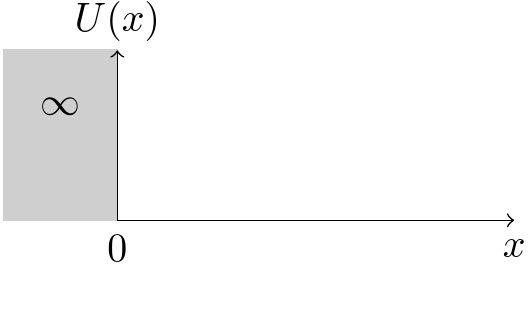
\includegraphics[width=0.3\textwidth]{polubeskonacni_domen.png}
	\caption{}
	\label{fig:bolubeskonacni_domen}
\end{wrapfigure}



Преформулисаћемо га тако да потенцијална баријера није бесконачна, већ коначна. Самим тим, када решимо тај проблем, можемо касније да пустимо да висина баријере тежи бесконачности и бум, вратили смо се на првобитни проблем. С обзиром да нам потенцијална енергија сада изгледа овако
\begin{equation}
	U(x) = \left\{ \begin{array}{rcl}
		0 & \mbox{,}
		& x>0 \\ 
		U_0\in\R^+ & \mbox{,} & x\leq0
	\end{array}\right.
\end{equation}
или као на слици (\ref{fig:konacna_barijera}). Сада, имамо две могућности за опсег енергије: или је $E\in(0, U_0)$ или је $E>U_0$. Посматрамо први случај и то када је честица унутар баријере, то јест, $x\in(-\infty, 0)$. Шредингерова једначина онда има облик:

\begin{equation*}
	-\frac{\hb^2}{2m}\frac{d^2\psi}{dx^2}+U_0\psi=E\psi
\end{equation*}\par
Увођењем смене $\gamma^2\equiv\frac{2m(U_0-E)}{\hb^2}$ добијамо следећи облик диференцијалне једначине\footnote{Слично као код једначине (\ref{eqn:sred_k}), једначина (\ref{eqn:sred_gamma}) је јако карактеристична и константно се враћамо на њу. Из тог разлога где год се појави симбол $\gamma$(на предавањима се углваном обележава са капа: $\kappa$, али је мени то слово мало незграпно, јер јако личи на $k$, тако да га замењујем са гама), сматрамо да је на исти начин дефинисан}:
\boxedeq{\label{eqn:sred_gamma}\psi'' - \gamma^2\psi=0}
Тада решење једначине може се написати у облику:
\begin{equation}
	\psi(x)=Ae^{\gamma x} + Be^{-\gamma x}
\end{equation}
\begin{wrapfigure}{r}{0.3\textwidth}
	\centering
	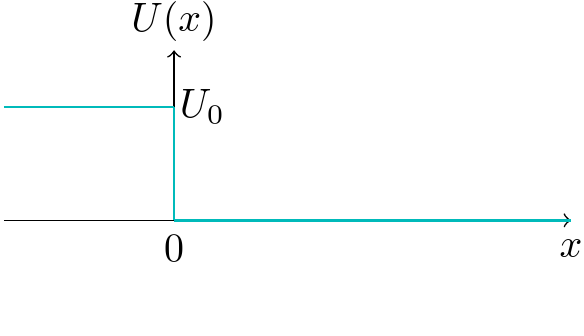
\includegraphics[width=0.3\textwidth]{konacna_barijera.png}
	\caption{}
	\label{fig:konacna_barijera}
\end{wrapfigure}\par
Како би уопште могли да нормирамо било коју функцију, она мора "нестати" (бити једнака нули) када $|x|\rightarrow\infty$. Пошто сагледавамо негативне вредности координате у овом случају, функција мора бити једнака нули када тежимо ка минус бесконачности. Одатле видимо да члан уз $B$ дивергира, тако да нам је први услов $B=0$.\par Ово доводи до мало чудног феномена. У класичној механици знамо да за потенцијал овог облика ми не бисмо имали решење за енергију унутар баријере, али овде оно постоји. Што је још бизарније, при почецима баријере таласна функција има ненулту вредност и како се удаљавамо од координатног почетка, све је мања и мања вероватноћа да наћемо честицу у том домену. Корак даље би било посматрање члана $\gamma$. Из дефиниције видимо да што је енергија ближа вредности $U_0$, то је фактор мањи, што само значи да што нам је енергија ближа том прагу, то је већа вероватноћа да ми наћемо честицу у баријери. Језиво...\par
Гурамо сада баријеру до бесконачности, то јест, $U_0\rightarrow\infty\implies\gamma\rightarrow\infty$. Због тога што нам је координата негативна нам следи да у лимесу $\psi\rightarrow0$. Ово ће нам послужити за касније јер знамо која је вредност функције у 0 (битно нам је ово јер функција мора бити непрекидна). Додатно, при оваквим трансформацијама, губимо један услов, а то је услов непрекидности првог извода (због бесконачног скока потенцијалне баријере).\par
Гледамо сада случај када је $x>0$. Разматрање је идентично случају који смо разматрали за слободну честицу на почетку, тако да можемо усвојити исто решење. Бирамо тригонометријски облик таласне функције.
\begin{equation*}
	\psi(x)=C\sin(kx) + D\cos(kx)
\end{equation*}
Из услова да $\psi(0)=0$ добијамо услов $D=0$. Феноменално! То значи да таласну функцију онда можемо да опишемо као
\begin{equation}
	\psi(x) = \left\{ \begin{array}{rcl}
		0 & \mbox{,}
		& x\leq0 \\ 
		C\sin(kx) & \mbox{,} & x>0
	\end{array}\right.
\end{equation}
Што значи да смо решили проблем? Одговор је: за мало... Ствар је што овако дефинисана таласна функција не може да се нормира \Sadey. Тако да враћамо се на стару добру технику - постављамо бесконачну баријеру од координате $L$ и касније је пуштамо да тежи бесконачности. Услов нормираности се онда своди на:
\begin{align*}
	&\int_{0}^{L}\norm{\psi(x)}^2dx = 1\\
	&C^2\int_{0}^{L}\sin^2(kx)dx=1\\
	&C^2\int_{0}^{L}\frac{1-\cos(2kx)}{2}dx=1\\
	&C^2\left[\frac{L}{2}-\frac{1}{4k}\sin(2kL)\right]=1\\
	&C^2\left[\frac{L}{2}-\frac{1}{2k}\sin(kL)\cos(kL)\right]=1\\
	&C^2\left[\frac{L}{2}-\frac{1}{2k}\cancelto{0}{\sin(kL)}\cos(kL)\right]=1\\
	&C^2\cdot\frac{L}{2}=1\implies C=\sqrt{\frac{2}{L}}
\end{align*}
У претпоследњем реду синус је нула јер представља таласну функцију на граници баријере, што знамо да је 0. Коначно, добијамо решење таласне функције
\begin{equation}\label{eqn:talasna_jed_polu_besk}
	\psi(x) = \left\{ \begin{array}{rcl}
		0 & \mbox{,}
		& x\leq0 \\ 
		\sqrt{\frac{2}{L}}\sin(kx) & \mbox{,} & x>0 \wedge L\rightarrow\infty
	\end{array}\right.
\end{equation}
Као и у претходним случајевима, док је $ $ коначно, спектар енергија је дискретизован. Једино у граничном случају добијамо континуални спектар.\par
\begin{mdframed}
	
\begin{zadatak}{Енергетски спектар слободне честице у полубесконачном домену}{}
	Одредити енергетски спектар таласне једначине (\ref{eqn:talasna_jed_polu_besk}).
\end{zadatak}
\begin{proof}[\unskip\nopunct]
Решење:\par
\lipsum[1-6]
\end{proof}

\end{mdframed}
\vspace{1em}
\hrule
\subsection*{Коначна јама са бесконачним зидовима}
\hrule
\vspace{1em}
Можда и најпознатији \textsf{\textit{mainstream}} проблем из квантне, на енглеском познат као \textbf{Particle in a box}. Овај проблем решавамо у једној просторној димензији, али лако може да се генерализује за 3D. Крећемо од тога да нам је дата потенцијална енергија следећег облика:
\begin{equation}
	U(x) = \left\{ \begin{array}{rcl}
		0 & \mbox{,}
		& x\in(0,d) \\ 
		\infty & \mbox{,} & x\notin(0,d)
	\end{array}\right.
\end{equation}
Примећујемо да честица једино може да се нађе у задатом домену и да енергија честице мора бити већа од нуле. Постављамо Шредингерову једначину на стандардан начин у домену где је потенцијална енергија 0.
\boxedeq{\kpsi}
Решење записујемо у тригонометријском облику
\begin{equation}\label{eqn:psi_trig}
	\psi(x) = A\sin(kx) + B\cos(kx)
\end{equation}
Због непрекидности таласне функције знамо $0=\psi(0^-)=\psi(0^+)=\psi(0)$ тако да из једначине (\ref{eqn:psi_trig}) следи да је $B=0$. Сада посматрамо таласну функцију на другој баријери, у $x=d$.
\begin{align*}
	&0=\psi(d^+)=\psi(d^-)=\psi(d)&\\
	\implies &A\sin(kd) = 0&\\
	\implies &kd = n\pi,&n\in\N
\end{align*}
Последњи ред није у потпуности математички тачан ($n$ би требало да буде елемент скупа $\Z$), али постоји разлог због тога што је баш овако изабран. Прво, $n=0$ би био тривијалан случај где или не постоји јама или је енергија једнака нули. Друго, с обзиром да су $k$ и $d$ позитивни, следи да $n\nless0$. Ако квадрирамо последњу релацију и изразимо енергију, добијамо\footnote{Приметимо да разлика између суседних енергија $\Delta E_n = E_n - E_{n-1}\sim \frac{1}{d^2}$. Ако би се баријера бесконачно удаљавала, то јест, $d\rightarrow\infty$, суседне енергије су све ближе и у граничном случају добијамо континуалан спектар исти оном који смо добили у претходном проблему.}
\begin{equation}\label{eqn:energija_kvantne_jame}
	E_n = \frac{n^2\pi^2\hb^2}{2md^2}
\end{equation}
Додатно, можемо да заменимо последњу релацију у нашу таласну једначину и онда добијамо решење
\begin{equation}
	\psi(x) = \left\{ \begin{array}{rcl}
		0 & \mbox{,}
		& x\notin(0,d) \\ 
		A\sin(\frac{n\pi}{d}x) & \mbox{,} & x\in(0,d)
	\end{array}\right.
\end{equation}\par
Једино што је остало је да одредимо константу $A$. То одрећујемо преко услова нормираности таласне функције.
\begin{align*}
	\int_{-\infty}^{\infty}\norm{\psi(x)}^2dx=1\\
	A^2\int_{0}^{d}\sin^2(\frac{n\pi}{d}x)dx=1\\
	A^2\cdot\frac{d}{2}=1\implies A=\sqrt{\frac{2}{d}}
\end{align*}\par
\begin{wrapfigure}{L}{0.3\textwidth}
	\centering
	\label{fig:beskonacna_simetricna_jama}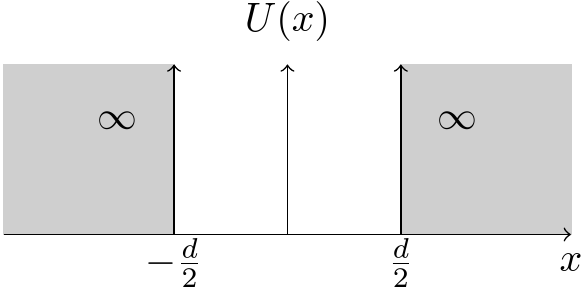
\includegraphics[width=0.3\textwidth]{beskonacna_jama.png}
	\caption{Бесконачна симетрична потенцијална јама}
\end{wrapfigure}
Посматрамо сада идентичан проблем, само са помереним потенцијалом тако да се јама налази у интервалу $x\in(-\frac{d}{2},\frac{d}{2})$. Питање је сада да ли ћемо добити другачије решење и због чега би било ко нормалан променио проблем након што га је решио\footnote{Одговор је наравно не, решење остаје исто. Разлог за то је нешто што толико није обраћено у курсу, а то су инваријантности Шредингерове једначине под одрећеним трансформацијама. У овом случају имамо само транслацију координате, али у општем случају то може да се докаже за Галилејеву трансформацију. За додатно објашњење погледати материјал на овом  \href{https://en.wikipedia.org/wiki/User:Likebox/Schrodinger\#Galilean_invariance}{линку}}. Одговор лежи заправо у својству које се манифестује код таласних функција када имамо симетричну потенцијалну енергију.


\begin{tcolorbox}[
	colframe=black,colback=red!35!white]\label{box:paran_potencijal}
	Ако је потенцијална енергија парна функција, онда су таласне функције или парне или непарне.
\end{tcolorbox}
С обзиром да нам је потенцијална коначна једино на интервалу $\left(-\frac{d}{2}, \frac{d}{2}\right)$, на том једино домену ћемо решавати Шредингерову једначину. Решавање се своди на исти случај као код једначине (\ref{eqn:sred_k}), тако да нам је решење у облику
\begin{equation}
	\psi(x) = A\sin(kx) + B\cos(kx)
\end{equation}
Према услову о парности потенцијалне енергије, разматраћемо засебно парна и непарна решења.\par
Посматрајмо прво парна решења. Таласна функција је онда облика $\psi_p(x) = B_p\cos(kx)$. Из услова непрекидности знамо да $\psi_p\left(\frac{d}{2}\right)=0$. Одатле следи да $$\cos\left(k\frac{d}{2}\right)=0$$то јест, $$k_p=\frac{(2p-1)\pi}{d}$$\par Ако изразимо енергију преко новодобијеног $k_p$
\begin{equation}\label{eqn:energija_parnih_stanja_kvantne_jame}
	E_p = \frac{(2p-1)^2 \pi^2 \hb^2}{2md^2}
\end{equation}
Примећујемо да ова енергија одговара енергији из једначине (\ref{eqn:energija_kvantne_jame}) за непарне вредности $n$.
\newpage
\section{Предавање - 10.3.2023.}
\section{Предавање - 22.3.2023.}
\section{Предавање - 24.3.2023.}
\section{Предавање - 29.3.2023.}
\section{Предавање - 5.4.2023.}
\section{Предавање - 7.4.2023.}
\section{Предавање - 12.4.2023.}





\appendix
\section{Струја вероватноће}

\section{Услов нормираности}\label{sec:uslov_normiranosti}
Услов нормираности се своди на услов да je функција $f$ квадратно интеграбилна: \begin{equation*}
	\int_{-\infty}^{\infty}|f|^2dx<\infty
\end{equation*}
али тако да је на целом пољу $\R$ једнака 1. То произилази из Копенхагенове интерпретације квантне механике: "\textit{$\norm{\psi}^2dx$ представља вероватноћу да се честица налази у домену $dx$, тако да честица се сигурно налази негде на целом простору}". 
С обзиром да је Шредингерова једначина хомогена, решење ће нам увек бити нека функција $g$ поможена са неком константном $A$ тако да када одредимо интеграл од $|g|^2$, рецимо да је вредност интеграла $I$, потребно је само да поставимо $A=\frac{1}{\sqrt{I}}$. Прецизније, константа је одређена на овај начин до неког мултипликативног фактора $e^{i\alpha}$, где је $\alpha$ неки реалан број. Овај фактор се занемарује јер, иако то мења облик таласне функције са математичког аспекта, физички смисао остаје исти, јер ће при поновном нормирању да се изгуби. Због претходне дискусије увек узимамо да је $A$ реална позитивна константа.

\end{document}